\section{Cubic spline interpolation}
	\begin{frame}{Cubic spline interpolation}
		\begin{block}{}
			\begin{itemize}
				\item $s_{j}$ on $[x_{j},x_{j+1}] \rightarrow$ cubic polinomial:
                $\newline \ \ \ s_{j}(x)=a_{j}+b_{j}(x-x_{j})+c_{j}(x-x_{j})^{2}+
                d_{j}(x-x_{j})^{3}$
                \item $s_{j}x=f(x_{j})(=s_{j-1}(x-j))$
                \item $s_{j}(x_{j+1})=s_{j+1}(x_{j+1})$
                \item $s^{'}_{j}(x_{j+1})=s^{'}_{j+1}(x_{j+1})$
                \item $s^{''}_{j}(x_{j+1})=s^{''}_{j+1}(x_{j+1})$
			\end{itemize}
		\end{block}
        \begin{figure}[h]
			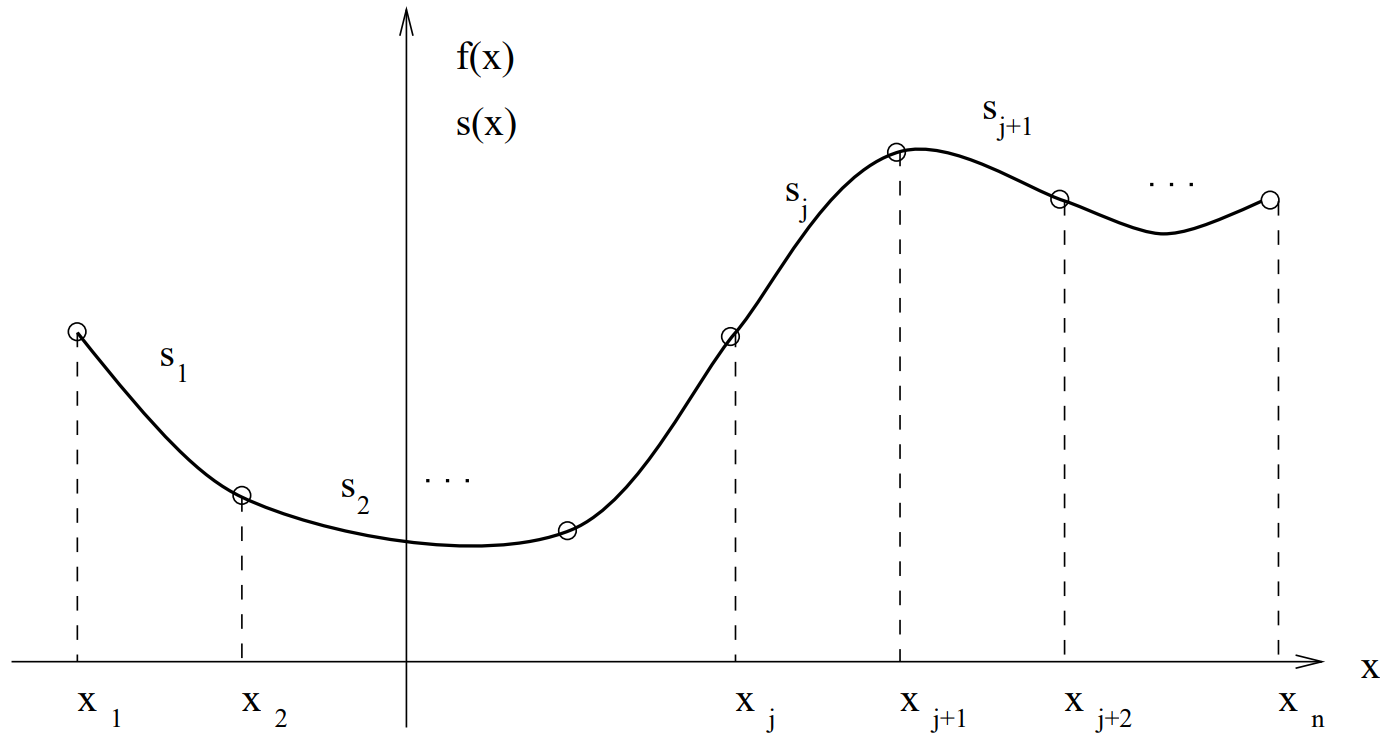
\includegraphics[width=.55\linewidth]{img/4/spline_img_4}
		\end{figure}
	\end{frame}